\documentclass{article}

\usepackage{amsmath, amsthm, amssymb, amsfonts}
\usepackage{thmtools}
\usepackage{graphicx}
\usepackage{setspace}
\usepackage{geometry}
\usepackage{float}
\usepackage{hyperref}
\usepackage[utf8]{inputenc}
\usepackage[english]{babel}
\usepackage{framed}
\usepackage[dvipsnames]{xcolor}
\usepackage{tcolorbox}

\colorlet{LightGray}{White!90!Periwinkle}
\colorlet{LightOrange}{Orange!15}
\colorlet{LightGreen}{Green!15}
\colorlet{LightBlue}{Blue!15}
\colorlet{LightRed}{Red!15}



\newcommand{\HRule}[1]{\rule{\linewidth}{#1}}
\newcommand{\N}{\mathbb{N}}
\newcommand{\R}{\mathbb{R}}



\declaretheoremstyle[name=Theorem,]{thmsty}
\declaretheorem[style=thmsty,numberwithin=section]{theorem}
\tcolorboxenvironment{theorem}{colback=LightGray}

\declaretheoremstyle[name=Proposition,]{prosty}
\declaretheorem[style=prosty,numberlike=theorem]{proposition}
\tcolorboxenvironment{proposition}{colback=LightOrange}

\declaretheoremstyle[name=Definition,]{definsty}
\declaretheorem[style=definsty,numberlike=theorem]{definition}
\tcolorboxenvironment{definition}{colback=LightGreen}

\declaretheoremstyle[name=example,]{examsty}
\declaretheorem[style=examsty,numberlike=theorem]{example}
\tcolorboxenvironment{example}{colback=LightRed}

\declaretheoremstyle[name=remark,]{Remarksty}
\declaretheorem[style=Remarksty,numberlike=theorem]{remark}
\tcolorboxenvironment{remark}{colback=LightBlue}

\setstretch{1.2}
\geometry{
    textheight=9in,
    textwidth=5.5in,
    top=1in,
    headheight=12pt,
    headsep=25pt,
    footskip=30pt
}

% ------------------------------------------------------------------------------

\begin{document}

% ------------------------------------------------------------------------------
% Cover Page and ToC
% ------------------------------------------------------------------------------

\title{ \normalsize \textsc{}
		\\ [2.0cm]
		\HRule{1.5pt} \\
		\LARGE \textbf{\uppercase{Analysis}
		\HRule{2.0pt} \\ [0.6cm] \LARGE{Study Note} \vspace*{10\baselineskip}}
		}
\date{}
\author{\textbf{Author} \\ 
		Sam Ren \\
		Grinnell College \\
		\today }

\maketitle
\newpage

\tableofcontents
\newpage

% ------------------------------------------------------------------------------
\section{Words before the text}
In the world of mathematics that full of abstruct terms and concepts.
We know that the real number is the fundation of all the mathematics. The real number is a set that contains all the rational numbers and irrational numbers.
The real number is a complete set, which means that it is a set that contains all the limit points of all the sequences.
It is important because it is the fundation of all the mathematics.
However, the real number is not enough for us to do the analysis. We need to define the limit, the continuity, the derivative, the integral, and so on.
Hence the basic structure of this note will be:
\begin{enumerate}
  \item Define the natural number, the integer, the rational number, and the real number.
   Explore the properties of them.
\item Define the limit, the continuity, the derivative, the integral, and so on.

\end{enumerate}
\section{Pre-knowledge}










\section{Numbers}
\subsection{The Natural Numbers}
\subsection{The Peano Axioms}
The natural number consist with set $\N$, where a distinguished element 0 $\in \N$, and a function $\nu : \N \to \N^{\times}:=\N \backslash \{0\}$ with following properties:
\begin{enumerate}
	\item $\nu$ is injective
	\item If a subset $N$ contains 0 and $\nu(n)\in N$ for all $n\in N$ then $N=\N$ 
\end{enumerate}

And we denote 






\section{Real analysis}
\subsection{Construction of the real numbers}
We are going to talk about the construction of real number system from rational number system. We know that the rational number system is not complete, which means that there are some points in the rational number system that cannot be represented by a rational number.
For example, $\sqrt{2}$ is an irrational number, which means that it cannot be represented by a rational number.
In order to construct the real number system, we need to add some points to the rational number system.
These points are called irrational numbers. The real number system is constructed by adding all the irrational numbers to the rational number system.
The real number system is a complete number system, which means that it contains all the limit points of all the sequences.
The real number system is the foundation of all the mathematics. It is the most important number system in mathematics.
The real number system is a complete number system, which means that it contains all the limit points of all the sequences.
The real number system is the foundation of all the mathematics. It is the most important number system in mathematics.
The real number system is a complete number system, which means that it contains all the limit points of all the sequences. The real number system is the foundation of all the mathematics. It is the most important number system in mathematics. The real number system is a complete number system, which means that it contains all the limit points of all the sequences. The real number system is the foundation of all the mathematics. It is the most important number system in mathematics. The real number system is a complete number system, which means that it contains all the limit points of all the sequences. The real number system is the foundation of all the mathematics. It is the most important number system in mathematics. The real number system is a complete number system, which means that it contains all the limit points of all the sequences. The real number system is the foundation of all the mathematics. It is the most important number system in mathematics. The real number system is a complete number system, which means that it contains all the limit points of all the sequences. The real number system is the foundation of all the mathematics. It is the most important number system in mathematics. The real number system is a complete number system, which means that it contains all the limit points of all the sequences. The real number system is the foundation of all the mathematics. It is the most important number system in mathematics. The real number system is a complete number system, which means that it contains all the limit points of all the sequences.
\subsubsection{Completeness of Real number}

Can you prove the "irrationality property" for the following set of numbers?

We know $\sqrt{2}$ is irrational. We need to prove that the set 
$L = \{ x \leq 0 \} \cup \{ x > 0 : x^2 < 2 \}$, 
together with the set $R = \{ r > 0 : r^2 > 2 \}$, 
are disjoint subsets of the rational numbers $\mathbb{Q}$, 
and that for every $r \in R$ there exists a "gap", 
i.e., there is no number in $L$ such that it is one less than any number in $R$. 
Formally, this is described as: for every $x \in (-\infty, \sqrt{2})$ 
and $(\sqrt{2}, +\infty)$, there is no rational number equal to $\sqrt{2}$.

Here are the conditions for a set $A$ and $B$ to prove the irrationality property, 
with $A$ and $B$ being nonempty subsets of $\mathbb{Q}$, disjoint and open:

\begin{enumerate}
  \item If $a \in A$, then there exists an $a' \in A$ such that $a' > a$.
  \item If $b \in B$, then there exists a $b' \in B$ such that $b' < b$.
  \item If $a \in A$ and $b \in B$, then $a \leq b$.
  \item There are no largest or smallest elements in $A$ or $B$.
\end{enumerate}

Since $L = A \cap \mathbb{Q}$ and $R = B \cap \mathbb{Q}$ are nonempty and consist of all rational numbers less than or equal to $\sqrt{2}$ and greater than $\sqrt{2}$ respectively, then according to the property above, we can define the set $A = (-\infty, \sqrt{2}) \cap \mathbb{Q}$, $B = (\sqrt{2}, +\infty) \cap \mathbb{Q}$.

Therefore, for $a \in A$ and $b \in B$, we have $a \leq x < \sqrt{2} < b$. Finally, since $A = (-\infty, x)$ and $B = [x, +\infty)$.







\clearpage
\subsection{Order properties of the real numbers}
\clearpage

\subsection{Sequences}
\subsection{Supremum \& Infimum}

\begin{definition}
	For a subset $M\subseteq \R$, $b\in \R$ is called Upper bound iff:
	\begin{equation*}
		\forall x\in M: x\leq b
	\end{equation*}
	If it is a lower bound, then $x\geq b$
\end{definition}

In simpler terms, an upper bound is a value that is greater than or equal to every element in the set.

\begin{definition}
	For a subset $M\subseteq \R$, $s\in \R$ is called supremum iff:
	\begin{itemize}
		\item $\forall x\in M: x\leq s$
		\item $\forall \varepsilon >0, \exists \bar{x}\in M : s-\varepsilon< \bar{x}$
	\end{itemize}
	Then we write $\sup M := s$
\end{definition}



\begin{definition}
		For a subset $M\subseteq \R$, $l\in \R$ is called infimum iff:
	\begin{itemize}
		\item $\forall x\in M: x\geq l$
		\item $\forall \varepsilon >0, \exists \bar{x}\in M : l+\varepsilon> \bar{x}$
	\end{itemize}
	Then we write $\inf M := l$
\end{definition}

\begin{remark}
	If $M$ is not bounded, then we write $\sup M:= \infty, \inf M:=-\infty $.
	
	If $M$ is an empty set, then we write $\sup M:= -\infty, \inf M:=\infty$
\end{remark}





%-------------------------------------------------------------------------
\subsection{Limits of Sequence}
\begin{definition}{Limit of Sequence}
The limit of a sequence $(a_n)$ is defined as follows: $\forall \varepsilon > 0, \exists N$ such that for all $n > N$,
\begin{equation*}
|a_n - L| < \varepsilon
\end{equation*}
The limit of the sequence is $L$, denoted as $\lim_{n\to \infty}a_n = L$.
\end{definition}
Here is an illustration of this definiton:
\begin{figure}[h]
	\centering
	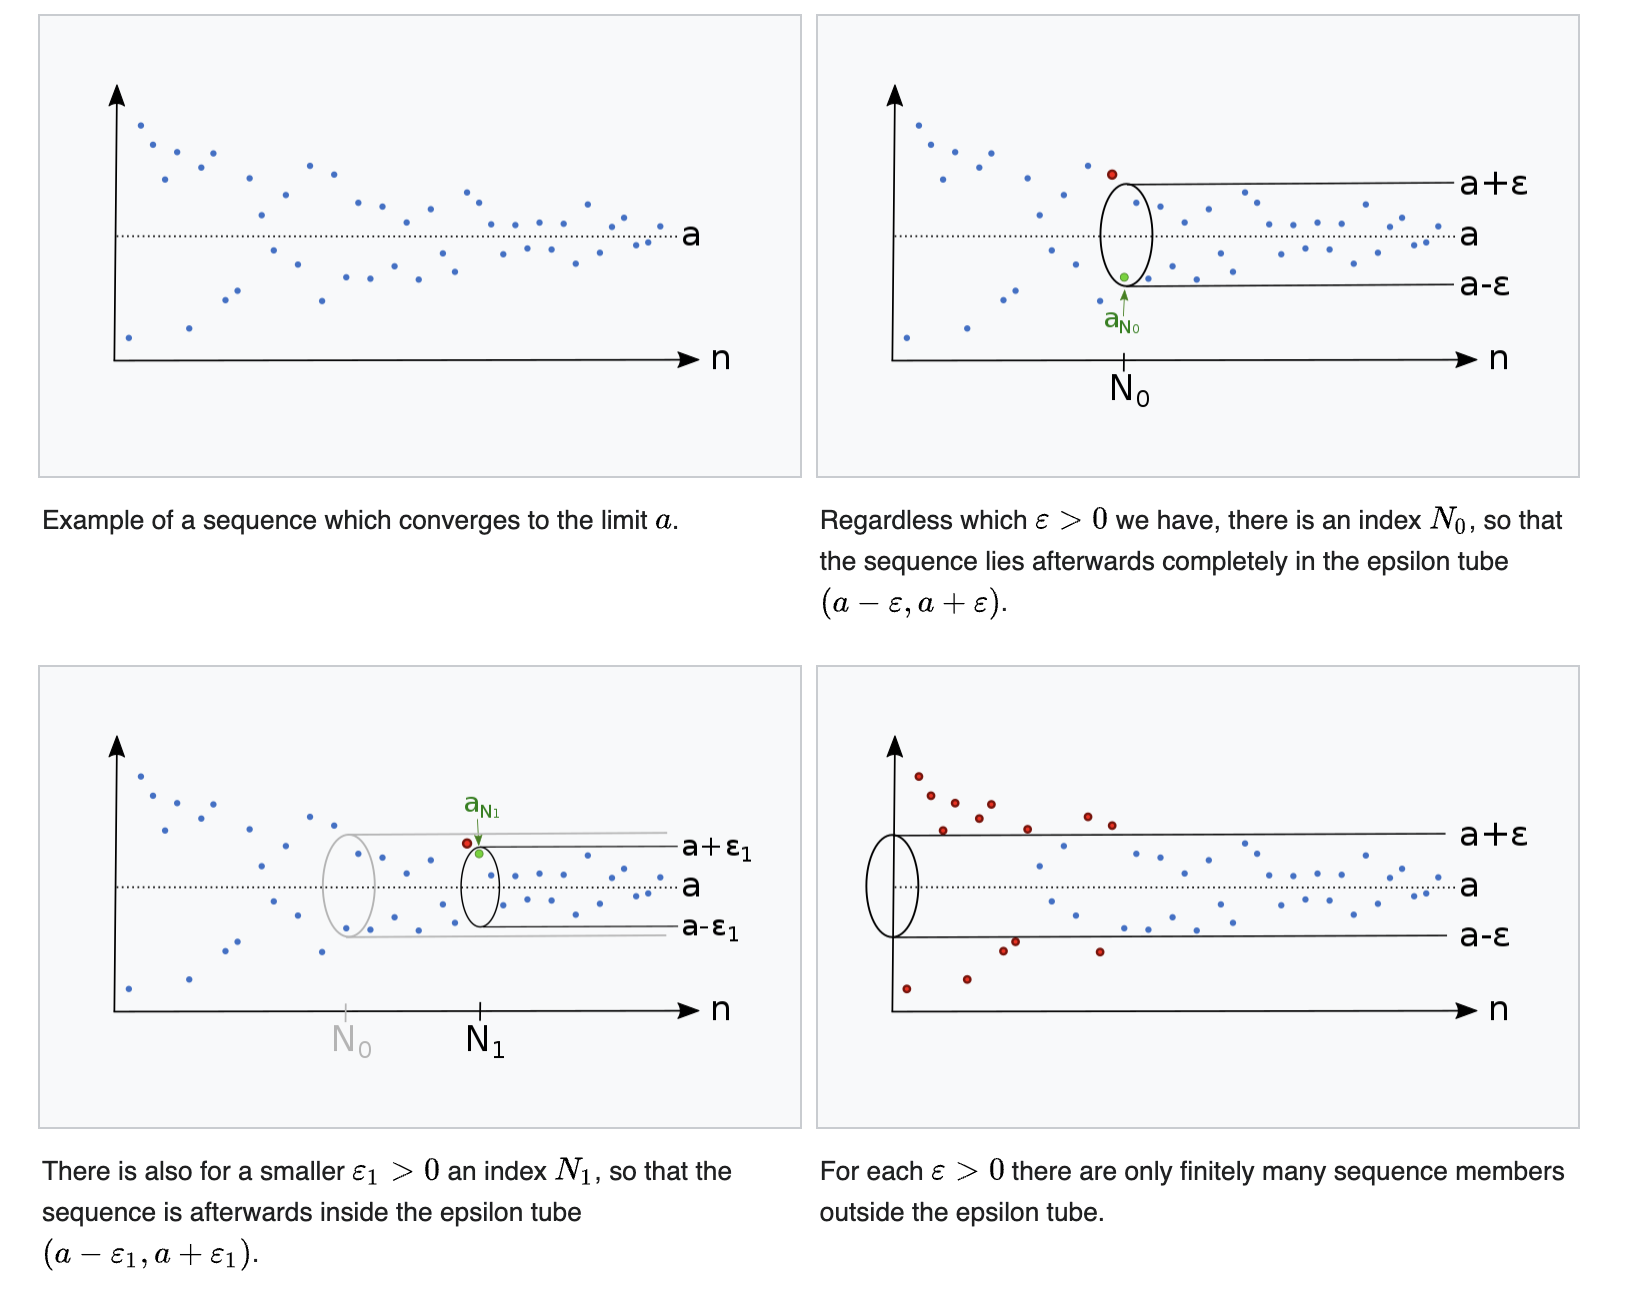
\includegraphics[scale=0.35]{img/seqlimit.png}
\end{figure}


If a sequence $(a_n)$ has a limit, then it is a convergent sequence; otherwise, it is a divergent sequence.

\begin{theorem}
The limit of a sequence possesses several important properties, including:
\begin{enumerate}
\item The limit of a sequence is unique.
\item If $a_n \leq b_n$ for all $n$ greater than some $N$, and both sequences have finite limits, then $\lim_{n\to \infty}a_n \leq \lim_{n\to \infty}b_n$.
\end{enumerate}
\end{theorem}

For further exploration: If $a_n > 0$ for all $n > N$, and the limit of $a_n$ as $n$ approaches infinity exists and is finite, then this limit is greater than 0.




\subsection{Cauchy sequence}\label{Cauchy sequence}

\begin{definition}
	A sequence $(a_n)_{n\in \mathbb{N}}$ is called cauchy sequence iff:
	\begin{equation*}
		\forall \varepsilon >0, \exists N\in \mathbb{N}, \forall n,m\geq N: |a_n-a_m|<\varepsilon
	\end{equation*}
\end{definition}

In simpler terms, this means that as you move further along in the sequence, the difference between its terms becomes smaller and smaller, eventually becoming as small as you like. 
\begin{remark}
	In real numbers, every convergent sequence is a Cauchy sequence, and every Cauchy sequence is convergent. This equivalence is a cornerstone of real analysis.
	\begin{equation*}
		\text{Cauchy sequence} \Leftrightarrow \text{Convergent sequence}
	\end{equation*}
	Which is known as completeness axiom.
\end{remark}

\begin{theorem}
	Dedekind completeness: 
	\begin{itemize}
		\item If $M\subseteq \R$ is upper bounded, then $\sup M\in \R$ exists
		\item If $M\subseteq \R$ is lower bounded, then $\inf M\in \R$ exists
	\end{itemize}
\end{theorem}

\begin{proof}
	Not yet understand()
\end{proof}

\begin{theorem}
	If a sequence is monotonically decreasing and bounded below, then it is a convergent sequence.
\end{theorem}


\subsection{Subsequence and Accumulation value}

\begin{definition}
	Let sequence $(n_k)$ be a strict monotomically increase sequence(that is $\forall k, n_{k+1}>n_k$). Then $(a_{n_k})_{k\in \N}$ is called a subsequence of $(a_n)_{n\in \N}$
\end{definition}

If the sequence is convergent then every subsequence of it is convergent to the same value.

\begin{definition}
	Accumulation value of $(a_n)_{n\in \N}$ is the limit value of subsequence $(a_{n_k})_{k\in \N}$.
\end{definition}

\subsection{Bolzano-Weierstrass Theorem}
\begin{theorem}
	If $(a_n)_{n\in \N}$ is bounded, then it has a accumlation value. In another word, every bounded sequence in real number has a convergent subsequence.
\end{theorem}

\begin{proof}
	Lets define a new sequence which has lower bound $c_0$ and upper bound $d_0$. Then we can esaily divide it into bisection with two same interval. 
	
\textbf{Bisection step:}	At least one of these subintervals must contain infinitely many terms of the sequence \((a_n)\). Label this subinterval as \([c_1, d_1]\). Repeat this process for \([c_1, d_1]\), dividing it into two and selecting the subinterval, say \([c_2, d_2]\), that contains infinitely many terms of \((a_n)\). Continue this process indefinitely. In each step, select a subinterval \([c_k, d_k]\) that contains infinitely many terms of the sequence. 

\textbf{Limit step} After we get the $[c_k,d_k]$, we can see that, $[c_k, d_k]\subset [c_{k-1}, d_{k-1}]\subset [c_{k-2}, d_{k-2}]\subset ...\subset [c_0, d_0]$. Hence, $d_1-c_1=\frac{1}{2}(d_0-c_0),d_n-c_n=\frac{1}{2^n}(d_{n-1}-c_{n-1})$. When $n\to \infty$, the difference apporach to 0. 

\textbf{Construction step:} It is obvious that $(c_n)_{n\in \mathbb{N}}$ is monotonically increase and $(d_n)_{n\in \mathbb{N}}$ is monotonically decrease. That is, they are convergent. (After prove they are convergent we can apply limit on these sequences) Notice:
\begin{equation*}
	\lim_{n\to \infty}(d_n-c_n)=0=\lim_{n\to \infty}(d_n)-\lim_{n\to \infty}(c_n)
\end{equation*}

\textbf{Final step:} Then let's define $(a_{n_k})_{k\in \mathbb{N}}$ as a new sequence where $a_{n_k}\in [c_k,d_k]$. That is:
\begin{equation*}
	c_k\leq a_k\leq d_k
\end{equation*}
By sandwich theorem we know that $(a_{n_k})_{k\in \mathbb{N}}$ is convergent.

\end{proof}


\subsection{Limit superior and inferior}
\begin{equation*}
	\begin{aligned}
		&\lim_{n\to \infty}a_n=\infty \Leftrightarrow \text{Divergent to }\infty \Leftrightarrow  \forall C>0, \exists N\in \mathbb{N}, \forall n\in N: a_n>C\\
		&\lim_{n\to \infty}a_n=-\infty \Leftrightarrow \text{Divergent to }-\infty \Leftrightarrow  \forall C<0, \exists N\in \mathbb{N}, \forall n\in N: a_n<C
	\end{aligned}
\end{equation*}

We call this type of accumulation as improper accumulation. When it does not bounded lower, then it has improper value of $-\infty$, when it does not bounded above, then it has improper value of $\infty$.

\begin{definition}
	For sequence $(a_n)_{n\in \mathbb{N}} $, An element $a\in \R \bigcup \{-\infty,\infty \}$ is called:
	\begin{itemize}
		\item Limit superior of $(a_n)_{n\in \mathbb{N}} $ if $a$ is the largest (improper) accumulation value of $(a_n)_{n\in \mathbb{N}} $. We write: $a=\limsup_{n\to \infty}a_n$
		\item Limit inferior of $(a_n)_{n\in \mathbb{N}} $ if $a$ is the smallest (improper) accumulation value of $(a_n)_{n\in \mathbb{N}} $. We write: $a=\liminf_{n\to \infty}a_n$
	\end{itemize}
	At the same time we can write:
	\begin{equation*}
		\limsup_{n\to \infty}a_n=\lim_{n\to \infty}\sup\{a_k | k\geq n \}
	\end{equation*}
		\begin{equation*}
		\liminf_{n\to \infty}a_n=\lim_{n\to \infty}\inf\{a_k | k\geq n \}
	\end{equation*}
\end{definition}

There are serval researons for define the limit superior and limit inferior
\begin{itemize}
	\item For sequences that do not converge, the limit superior and inferior provide a way to describe their behavior. They are particularly useful in handling oscillating sequences or sequences with multiple limit points. 
	\item Unlike the usual limit, the limit superior and limit inferior always exist for any bounded sequence and for many unbounded sequences.
	\item If a sequence $a_n$ does converge, then its limit superior and limit inferior are both equal to this limit. This property is often used in proofs to show convergence.
	\item These concepts are also used in the convergence tests for series, particularly in understanding the behavior of the terms of a series.
\end{itemize}

\begin{example}
	\begin{equation*}
		a_n=(-1)^n\cdot n= -1,2,-3,...
	\end{equation*}
	It is obvious that this sequence is not convergent however we can find a subsequence where we can esaily get the limit superior and inferior:
	\begin{equation*}
		\limsup_{n\to \infty}a_n=\infty
	\end{equation*}
	\begin{equation*}
		\liminf_{n\to \infty}a_n=-\infty
	\end{equation*}
\end{example}

\begin{theorem}
	Sequence $a_n$ is conergent if:
	\begin{equation*}
		\limsup_{n\to \infty}a_n=\liminf_{n\to \infty}a_n \notin \{\infty,-\infty \}
	\end{equation*}
	At the same time, if $a_n$ is divergent to $\infty$ then:
	\begin{equation*}
		\limsup_{n\to \infty}a_n=\liminf_{n\to \infty}a_n=\infty
	\end{equation*}
\end{theorem}

Some properties which are only exists when the value is defined(Not infinty times zero etc.):
\begin{enumerate}
	\item $\limsup_{n\to \infty}(a_n+b_n)\leq \limsup_{n\to \infty}a_n+\limsup_{n\to \infty}b_n$
	\item $\limsup_{n\to \infty}(a_n\cdot b_n)\leq \limsup_{n\to \infty}a_n\cdot \limsup_{n\to \infty}b_n$
\end{enumerate}

For limit inferior, we just change the direction of inequality.
\clearpage
\subsection{Series}
\begin{definition}
Series are sequence($S_n$) which is the summation of a sequence $a_n$ from inital value to infinity, where we denote it as:
	\begin{equation*}
		S_n=\sum_{i=1}^n a_i,n\in \mathbb{N}
	\end{equation*}
	If $S_n$ is convergent then we write: 
	\begin{equation*}
		\sum_{i=1}^\infty a_i:=\lim_{n\to \infty} S_n=\lim_{n\to \infty}\sum_{i=1}^\infty a_i
	\end{equation*}
\end{definition}


\begin{example}
Harmonic series are special series which write as:
\begin{equation*}
	\sum_{k=1}^\infty \frac{1}{k}
\end{equation*}	
This serie seems to be convergent however it is not.
\end{example}

\begin{proof}
	Let $S_n=\sum_{k=1}^n \frac{1}{k}$ where increase monotonically and we are going to prove that this sequence is not bounded above. 
\end{proof}

Here are some properties if series $\sum a_k, \sum b_k$ are convergent
\begin{enumerate}
	\item $\sum(a_k+b_k)=\sum a_k  +\sum b_k$ convergent
	\item $\sum (\lambda a_k)=\lambda \sum a_k$
\end{enumerate}


\subsubsection{Criterion of Series}
\begin{definition}
	Absolute convergence: A series $\sum_k^{\infty}a_k$ is called absolute convergent iff $\sum_k^{\infty}|a_k|$ is convergent. When $\sum_k^{\infty}a_k$ is convergent and $\sum_k^{\infty}|a_k|$ is divergent then it is called conditional convergence.
\end{definition}


\begin{theorem}
	Cauchy criterion claims that a series in $\R$ is convergent iff it is cauchy sequence and follows that:
	\begin{equation*}
	\sum^\infty a_k \text{Convergent} \leftrightarrow \forall \varepsilon >0, \exists N\in \N, \forall n\geq m\geq N
	\end{equation*}
	we have:
	\begin{equation*}
		|\sum_m^n a_k|<\varepsilon
	\end{equation*}
	which it is simply another representation of cauchy sequence
\end{theorem}

\begin{theorem}
	$\sum_{k=1}^\infty a_k$ is convergent $\Rightarrow$ $(a_k)_{k\in \N}$ convergent and $\lim_{k\to \infty}a_k=0$
\end{theorem}
\begin{proof}
	$\forall \varepsilon >0,\exists
	N\in \N$ s.t. $\forall n,m\geq N$ there is $|s_n-s_m|<\varepsilon \Rightarrow |a_n+a_{n+1}+...+a_m|<\varepsilon$.
	
	Hence $|a_n-0|<|a_n+...+a_m|<\varepsilon$ therefore $\forall \varepsilon >0,\exists
	N\in \N$ s.t. $n\geq N$ and $|a_n-0|<\varepsilon$ it is the same of limit $\lim_{k\to \infty}a_k=0$ exists.
\end{proof}








\clearpage
\subsection{Introduction to topology}
\subsection{Open, Close, and Compact sets}
We first define what is a \textbf{neighborhood}:
\begin{definition}
	\begin{equation*}
		\varepsilon>0, (x-\varepsilon,x+\varepsilon):=B(x)
	\end{equation*}
	which we call it $\varepsilon$-neighborhood. A neighborhood of $x$ is:
	\begin{equation*}
		For\ M\subseteq \R, \exists \varepsilon>0, st. M\supseteq B(x)
	\end{equation*}
\end{definition}

\begin{definition}
	$M\subseteq \R$ is called \textbf{open set} in $\R$ iff for all $x\in M$, $M$ is a neighborhood of $x$.
	\begin{equation*}
		\forall x\in M,\exists \varepsilon>0, st. N(x)\subseteq M
	\end{equation*}
\end{definition}

After define what is open set we are going to define close set use the definition of opensets:
\begin{definition}
	A set $A$ is close set iff $A^{C}$ is open set
\end{definition}
	
 \begin{theorem}\label{Close and convergent}
 	A set is close can be deseribed by convergent sequence: For $A\in \R$ if all $(a_n)_{n\in \mathbb{N}}$ with $a_n\in A$ and $\lim_{n\to \infty}a_n\in A$ then $A$ is close set.
 \end{theorem}

Then we are going to give a special definition which are so important---compact set
\begin{definition}
	$A\subseteq\R$ is called compact if for all $a_n\in A,\forall n\in \mathbb{N}$ there is a convergent subsequence $a_{n_k}$ where:
	\begin{equation*}
		\lim_{k\to \infty}a_{n_k}\in A
	\end{equation*} 
\end{definition}

\begin{itemize}
		\item $\emptyset$ is compact
		\item $[c,d],c<d$ is compact
		\item $\{n \}$ is compact
		\item $\R$ is not compact
\end{itemize}

\begin{theorem}\label{Heine-Borel theorem}
	\textbf{Heine-Borel theorem:} For $A\subseteq \R$ is compact iff its bounded and closed 
\end{theorem}

\begin{proof}
	We will prove this equivlent statement in both direction:
	
	$(\Leftarrow):$ Use the same method in proof of Bolzano-Welerstrass theorem

	$(\Rightarrow)$ Assume $A$ is compact, then there is an convergent sequence $a_n\in A\subseteq \R$ where has accumulation value $\bar{a}\in A$. We first prove that $A$ is closed---because there is only one accumulation value $a$, hence $\bar{a}=a\in A$. By theorem \ref{Close and convergent} this means that $A$ is closed. We then prove that $A$ is bounded by contradiction---Assume $A$ is unbounded, then $\exists a_n\in A$ where $|a_n|>n,\forall n\in \mathbb{N}$, we constructed does not have any convergent subsequence. This is because its terms grow without bound and thus cannot converge to any point in $\R$. A sequence that tends to infinity doesn't converge, which contradicts the property of compactness in $A$.



\end{proof}

\subsection{Pointwise convergence and uniform convergence}
\begin{definition}
   A sequence of function($f_n$) is called Pointwise convergent to function $f:I\to \R$ iff:
   \begin{equation*}
   	\forall \bar{x}\in I,\forall \varepsilon >0, \exists N\in \N , \forall n\geq N, s.t. |f_n(\bar{x})-f(\bar{x})|<\varepsilon
   \end{equation*}
\end{definition}

In a similar way, we can define the uniform convergent of sequence of function:
\begin{definition}
	A sequence of function($f_n$) is called uniform convergent to function $f:I\to \R$ iff:
   \begin{equation*}
   	\forall \varepsilon >0, \exists N\in \N , \forall n\geq N, \forall \bar{x}\in I, s.t. |f_n(\bar{x})-f(\bar{x})|<\varepsilon
   \end{equation*}
\end{definition}

It is easy to see that the difference of defintion is simply exchange the order of $\forall \bar{x}\in I$, however it will alternate the meaning of the whole definiton and cause a totally different udnerstanding.

\begin{definition}
	Distance of two function $f(x),g(x)$ are defined as:
	\begin{equation*}
		\sup_{x\in I} |f(x)-g(x)|\equiv ||f-g||_{\infty}
	\end{equation*}
\end{definition}

By defining the distance of functions we can rewrite the definiton of uniform convergence:
\begin{equation*}
	 n\to \infty, ||f_n-f||_{\infty}\to 0
\end{equation*}

\begin{theorem}
	The relationship between pointwise convergence and uniform convergence are:
	\begin{itemize}
		\item pointwise convergence $\nRightarrow$ uniform convergence
		\item uniform convergence $\Rightarrow$ pointwise convergence
	\end{itemize}
\end{theorem}

\subsection{Limits of functions}
\begin{definition}
	Let $f: I \to \R, x_0\in I$ If there is $c\in \R$ and all sequence $(x_n)$ with $\lim_{n\to \infty}x_n=x_0$ we have ($f(x_n)$) is also convergent with $\lim_{n\to \infty}f(x_n)=C$ then we write:
	\begin{equation*}
		\lim_{x\to x_0,x_0\in \R}f(x)=C
	\end{equation*}
\end{definition}
Left and Right limit is an important tool for further exploration.
\begin{definition}
	(Right limit,$\lim_{x\to x_0^+}$)For function $f:I\to \R$, and $x_0\in I\cap (x_0,+\infty)$ is some adherent point, then we define the right limit of function at $x_0$ as:
	\begin{equation*}
		\lim_{x\to x_0,I\cap (x_0,+\infty)} f(x)
	\end{equation*}
	In short cut we write:
	\begin{equation*}
		\lim_{x\to x_0,(x_0,+\infty)}
	\end{equation*}
\end{definition}
In the similar way we define the left limit.


\subsection{Compactness and Continuity}
\begin{definition}
	Let $f: I \to \R$ be a function with $I \subseteq \R$. $f$ is called continuous at $x_0\in I$ if \begin{equation*}
		\lim_{x\to x_0}f(x)=f(x_0)
	\end{equation*}
	If $f$ is called continuous on $I$, if $f$ is continuous at $x_0$ for all $x_0\in I$. 
\end{definition}
If $f(x)$ is continuous $\forall x_0\in I$, then we have:
\begin{equation*}
	\lim_{n\to \infty}f(x_n) = f(\lim_{n\to \infty}x_n)
\end{equation*}

\begin{example}
	There is an important function:
	\begin{equation*}
		f(x)=\begin{cases}
			1&,x\in \mathbb{Q}\\
			0&,x\notin \mathbb{Q}
		\end{cases}
	\end{equation*}
	You should now that $\mathbb{Q}$ is dense in the real number field. That is, you can alwats construct a sequence where it convergent to a real number. You can choose a sequence that convergent to 1 when $x\to x_0$ also you can choose another sequence that convergent to 0 when $x\to x_0$. Hence $\lim_{x\to x_0}f(x)$ does not exists. The function is not continuous at any points.
\end{example}

This definiton of continuity is based on the concept of limit. However, there is a equivlence statement of continuous by using the traditional analytical language---$\varepsilon,\delta$ words.

A function is continuous at $x_0$ if
\begin{equation*}
	\forall \varepsilon >0,\exists \delta>0, \forall x\in I: |x-x_0|<\delta \Rightarrow |f(x)-f(x_0)|<\varepsilon
\end{equation*}

Let's proof the equivlence of two definiton:
\begin{proof}
	($\Rightarrow$) Assume $\exists \varepsilon >0,\forall \delta>0, \exists x\in I: |x-x_0|<\delta \Rightarrow |f(x)-f(x_0)|<\varepsilon$. Lets take $\delta=\frac{1}{n},n\in \N$. We have $\forall n\in \N$, $x_n\in I\backslash \{x_0\}$ with $|x_n-x_0|<\frac{1}{n}$ and $|f(x_n)-f(x_0)|\geq \varepsilon$. Therefore it is not continuous at $x_0$.\\
($\Leftarrow$) choose sequence $(x_n)\subseteq I\backslash \{x_0\}$ with limit $x_0$. Let $\varepsilon>0$ take $\delta>0$. there is $N\in \N$ such that for all $n\geq N$ we have $|x_n - x_0|<\delta$, also by assumption we have $|f(x_n)-f(x_0)|<\varepsilon$ therefore $f$ is continuous.
\end{proof}

\begin{theorem}
	For basic combination of two functions$f,g:I\to \R$: addition, Subtraction, mutiplication. If both $f,g$ are continuous at $x_0$ then all the result functions are continuous. For division,  the denominator should not be 0.
\end{theorem}

\begin{proof}
	Assume $f,g:I\to \R$ is continuous, then we have $	\lim_{n\to \infty}f(x_n) = f(\lim_{n\to \infty}x_n)$ and $	\lim_{n\to \infty}g(x_n) = g(\lim_{n\to \infty}x_n)$. Now for:
	\begin{itemize}
		\item $f+g=h$, we have $\lim_{n\to \infty}(f(x_n)+g(x_n))=\lim_{n\to \infty}(h(x_n))= f(\lim_{n\to \infty}x_n)+g(\lim_{n\to \infty}x_n)=h(\lim_{n\to \infty}x_n)$. 
		\item $f\cdot g=h$, we have $\lim_{n\to \infty}(f(x_n)\cdot g(x_n))=\lim_{n\to \infty}(h(x_n))= f(\lim_{n\to \infty}x_n)\cdot g(\lim_{n\to \infty}x_n)=h(\lim_{n\to \infty}x_n)$
	\end{itemize}
\end{proof}

What about composition of functions $f(g(x))$.
\begin{theorem}
	For two functions $f:I\to \R,g:J\to \R, I,J\subseteq \R $ with $g[J]\subseteq I$ and $g$ continuous at $x_0\in J$, $f$ continuous at $g(x_0)\in I$. Therefore we have $f(g(x)):J\to \R$ continuous at $x_0\in J$
\end{theorem}

\begin{proof}
	Choose sequence $(x_n)\subseteq J\backslash \{x_0\}$ with limit $x_0$
	\begin{equation*}
		\lim_{n\to \infty}(f\circ g)(x_n)=	\lim_{n\to \infty}f(g(x_n))=f(	\lim_{n\to \infty}g(x))=f(g(	\lim_{n\to \infty}x_n)))
	\end{equation*}
\end{proof}

Now lets talk about what is the relationship between compactness and continuous function on a real number field.

\begin{theorem}
	Let continuous function $f:I\to \R$ where $I$ is compact on $\R$(that is $I$ is bounded and closed by Heine-Borel Theorem). Then the image $f[I]$ is compact too. With the superior and inferior:
	\begin{equation*}
		f(x^+) := \sup \{f(x)|x\in \R\}
	\end{equation*}
	\begin{equation*}
		f(x^-) := \inf \{ f(x)|x\in \R \}
	\end{equation*}
\end{theorem}

Now lets look at the property of uniform convergent functions where the sequence of functions are all continuous:
\begin{theorem}
	Let $f_n:I\to \R$ be continuous for all $n\in \N$ and $f_n$ uniformly convergent to $f$. Then $f$ is continuous 
\end{theorem}

\begin{proof}
Let $\varepsilon>0, x>0,x\in I$\\ 
	Because $f_n$ is uniform convergent to $f$ therefore we have:
	\begin{equation*}
		\forall \varepsilon' >0, \exists N\in \N , \forall n\geq N, \forall {x}\in I, s.t. |f_n({x})-f({x})|<\varepsilon'
	\end{equation*}
	In this case, we are going to write the continuity condition of $f_N$ at $x_0$ down by finding $\delta>0$:
	\begin{equation*}
		|x-x_0|<\delta, \Rightarrow |f_N(x)-f_N(x_0)|<\varepsilon'
	\end{equation*}
	And now the condition of $f$ to be continuous is:
	\begin{equation*}
	\begin{aligned}
		|f(x)-f(x_0)| &=|f(x)+f_N(x)-f_N(x_0)+f_N(x_0)-f_N(x)-f(x_0)|\\
		&\leq|f(x)-f_N(x)| + |f_N(x)-f_N(x_0)|+|f_N(x_0)-f(x_0)|\\
		&< \varepsilon'+\varepsilon'+\varepsilon'=\varepsilon
		\end{aligned}
	\end{equation*}
	(Explaination: for first and third term, it is given by the uniform convergence and second term is the continuity of $f_N$)Therefore, by choosing $\varepsilon'=\frac{\varepsilon}{3}$, we can show that the function $f$ is continuous.
\end{proof}
Now we shall introduce a very important theorem which are useful---Intermediate Value Theorem

\begin{theorem}
	Let $f:[a,b]\to \R$ be a continuous function and $y\in [f(a),f(b)]$ or $y\in [f(b),f(a)]$, the Intermediate Value Theorem tells us there is $\bar{x}\in [a,b]$ with $y=f(\bar{x})\in [f(a),f(b)]$.
\end{theorem}

\begin{proof}
	
\end{proof}

\subsubsection{Some continuous functions}\label{contfunc}
Now I am going to list out serval important continuous functions:
\begin{example}
	exp$:\R\to\R$ is continuous function defined by $\exp(x)=\sum_{k=0}^\infty \frac{x^k}{k!}$. And we define $e$ the constant as $e:=\exp(1)$. You may know another equivlent definition of this constant given by the limit:
	\begin{equation*}
		e=\lim_{n\to \infty}(1+\frac{1}{n})^n
	\end{equation*}
	Here are some basic properties:
	\begin{itemize}
		\item $\exp(x+y)=\exp(x)\times\exp(y)$
		\item $\exp(x)=e^x$
		\item $\lim_{n\to \infty}\exp(n)=\infty$,$\lim_{n\to -\infty}\exp(n)=0$
		\item $\exp : \R \to (0,\infty)$ is bijection with inverse we called the logarithm function.
	\end{itemize}
	We just mentioned Logarithm function, which is the inverse function of exp function:
	\begin{equation*}
		\exp(y)=x\Rightarrow y=\log(x)
	\end{equation*}
\end{example}






\subsection{Differentiation}
In order to further understand the features of functions, we need to know the rate of change of them. In this case, we shall introduce a new concept---differentitation
\begin{definition}
For function $f:I\to \R$ where $I\in \R$ and a limit point($x_0$) of $I$. Now we define a function $f'(x)$ as:
\begin{equation*}
	\lim_{x\to x_0,x_0\in I\backslash \{x_0\}} \frac{f(x)-f(x_0)}{x-x_0}
\end{equation*}
If this limit convergent to $L\in \R$. Then we call the function is differentiable at $x_0\in I$ with derivative $L$. That is $f'(x_0):=L$
\end{definition}

It is obvious that only smooth function are differentiable. Now here are some examples:
\begin{example}
	For function $f(x)=|x|$ by definition the derivative at 0 is:
	\begin{equation*}
		\lim_{x\to 0}\frac{f(x)-f(0)}{x-0}=\lim_{x\to 0,x\in \R \backslash \{0\}} \frac{|x|}{x}
	\end{equation*}
By take left and right limit of the function at 0 it is obvious that we will get 2 results: $\{1,-1\}$
\end{example}

\section{The mean value theorem}
We now shall talk about a baby version of Mean value theorem which named as Rolles theorem:
\begin{theorem}
   If funtion $f$ is a funtion where differentiable on $[a,b]$ and $f(a)=f(b)$ then there is $\bar{x}\in (a,b)$ where $f'(\bar{x})=0$
\end{theorem}
We shall now show a proof of this theorem:
\begin{proof}[Proof of Rolles theorem]
  By the extreme value theorem, we have $f$ has maximum and minimum value on $[a,b]$. If the maximum and minimum value are the same then we have $f$ is constant and $f'(\bar{x})=0$. If they are not the same,
  then we have $f$ has maximum and minimum value. Therefore there is $\bar{x}$ where $f'(\bar{x})=0$.
\end{proof}
Now we shall talk about the mean value theorem:
  \begin{theorem}[Mean value theorem]
We shall notice that we can rewrite the Rolles theorem as a special case of mean value theorem.
For function $f$ is a funtion where differentiable on $[a,b]$ then there is $\bar{x}\in (a,b)$
where $f'(\bar{x})=\frac{f(b)-f(a)}{b-a}$ and we can rewrite it as: $f'(\bar{x})=\frac{f(b)-f(a)}{b-a}$
\end{theorem}

\subsection{Talor series and Forier series}
In this subsection we are going to talk about two important series which are used to apporximate the functions by polynomial functions,
they are Talor series and Forier series. 
\begin{definition}[Talor series]
Talor series is a representation of a function as an infinite sum of terms that are calculated from the values of the function's derivatives at a single point.
Where in mathematiacl language, we write the Talor series of a function $f$ at point $x_0$ as: 
\begin{equation*}
  f(x)=\sum_{n=0}^\infty \frac{f^{(n)}(x_0)}{n!}(x-x_0)^n
  \end{equation*}
\end{definition}
While the $n$ gets larger, the approximation of the function gets better. However, the convergence of the series is not guaranteed.
It is because the function may not be smooth enough. 
Now we shall introduce the Forier series:
\begin{definition}[Forier series]
  Forier series is a way to represent a function as the sum of simple sine waves. The Forier series of a function $f$ is:
  \begin{equation}
    f(x)=a_0+\sum_{n=1}^\infty a_n\cos(nx)+b_n\sin(nx) 
  \end{equation}
\end{definition}
The reason why we use sine and cosine function is that they are orthogonal to each other.
Meanwhile the Forier series is guaranteed to converge to the function if the function is piecewise smooth.
Hence the Forier series is more powerful than the Talor series.
We can use Forier series to approximate the function which is not smooth enough.

And now we can talk about the theorem of these series:
\begin{theorem}
  Forier series is convergent to $f$ if $f$ is piecewise smooth.
  
\end{theorem}

\begin{proof}
  We can prove this theorem by using the Dirichlet's theorem.
  Where we can show that the partial sum of the Forier series is bounded.
\end{proof}


\subsection{Riemann integration}
we need to describe how one can partition a large interval into smaller intervals.
\begin{definition}
	A space $X\subseteq \R$ is called connected iff for any $x,y\in X$ and $x<y$ the bounded interval $[x,y]$ is always a subset of $X$. That is, in another word, every element in the interval is in $X$.
\end{definition}
It is obvious that: Connected and bounded space in $\R$ $\equiv$ bouneded interval in $\R$. 
Now we shall deine the length of an interval:
\begin{definition}
	(Length of interval), the length of interval $I$, such as $I=(a,b),(a,b],[a,b],[a,b)$ where $a<b$. We define the length of the interval $|I|$ as $b-a$. If $I=\emptyset$ or a point, then $|I|=0$
\end{definition}

Now we shall define the partitions:
\begin{definition}
	Let $I$ be bounded interval. A partition \textbf{P} of $I$ is a collection of bounded intervals contained in $I$. Where every $x\in I$ lies exactly one of the bounded interval $J$ in \textbf{P}  
\end{definition}

Now we shall discuss some property of length based on the partition:
\begin{theorem}
	(Length is finitely additive) for interval $I$ and its partition we have:
	\begin{equation*}
		|I| = \sum_{J\in \textbf{P}} |J|
	\end{equation*}
\end{theorem}

\begin{proof}
	You can prove this theorem by using induction
\end{proof}

Now we wonder how can we compare two partition of same interval:
\begin{definition}
	For interval $I$ we have \textbf{P} and $\textbf{P}^{'}$ as partition of it. We say \textbf{P} is finer than \textbf{P}$^{'}$ if $\forall J\in \textbf{P}, \exists K\in \textbf{P}^{'},s.t. \ J\subseteq K$
\end{definition}

This definition is very intuitive of the idea 'finer'. 
\begin{definition}
	We define the common refinement($\textbf{P}\#\textbf{P}^{'}$) of who paritions $\textbf{P},\textbf{P}^{'}$ as the set of intersection of partitions of an interval:
	\begin{equation*}
		\textbf{P}\#\textbf{P}^{'}:=\{K\cap J|K\in \textbf{P},J\in \textbf{P}^{'}\}
	\end{equation*}
\end{definition}

\begin{definition}
	A function is called piecewised function if for the function $f:I\to \R$,$I$ is bounded interval, the parition of $I$ is $P$, where for every $J\in P$, the $f$ is a constant. 
\end{definition}

Now lets get into the topic, which 'Integration' the concept first appear in this note:
\begin{definition}
	Let $I$ be a bounded interval, let $P$ be a partition of I. Let $f:I\to \R$ be a function which is piecewise constant with respect to $P$. Then we deine the piecewise constnt integral p.c. $\int_{[P]}f$ of $f$ with respect to the partition $P$ by the formula:
	\begin{equation*}
		p.c.\int_{[P]}f:=\sum_{J\in P}c_J|J|
	\end{equation*}
	Where for each $J$ in $P$, we let $c_J$ be the constant value of $f$ on $J$
\end{definition}


\begin{definition}
  For $$I=[a,b], a<b$$ we define the Riemann integral of a function $f:I\to \R$ as:
  \begin{equation}
    \int_a^b f(x)dx:=\sup\{p.c.\int_{[P]}f|P \text{ is partition of } I\} 
  \end{equation}
\end{definition}




\subsection{Introduction to measure theory}
\subsection{Lebesgue integration}
\subsection{Lebesgue measure}
\subsection{Relation to complex analysis}



\section{Complex analysis}
\subsection{Complex numbers and geometric interpretation}
\subsection{Complex functions}
\subsection{Riemann sphere}
\subsection{Complex Differentiation}
\subsection{The Logarithmic Function}
\subsection{Riemann surface}
\subsection{Complex Integration}























\subsection{Riemann Integral}
In the previous sections we have talked about the integral in general, now we are going to talk about the Riemann integral which is a special type of integral. 
\begin{definition}[Riemann integrable]
A function $f:I\to \R$ is called Riemann integrable on $I$ if there is a number $I$ such that for every $\varepsilon >0$,
there is a partition $P$ of $I$ such that for every refinement $P^{'}$ of $P$ we have $|I-\int_{[P^{'}]}f|<\varepsilon$ 

\end{definition}

This definition tells us that the Riemann integral is a limit of the piecewise constant integral.
where we can esaly prove that the Riemann integral is a linear operator. Meanwhile the Riemann integral is a continuous operator. 
The derivarive as we already know is the reverse operation of the integral. Hence Derivative is also a linear operator. 
This definition tells us the integrability of the function is based on the limit of the piecewise constant integral. 


Now we are going to talk about some property of the Riemann integral:
\begin{theorem}[Riemann integral is linear]
Riemann integral is a linear operator. That is for $f,g$ are Riemann integrable on $I$ and $a,b\in \R$ then we have:
$$\int_{I}(af+bg)=a\int_{I}f+b\int_{I}g$$
\end{theorem}

We shall now prove this theorem:

\begin{proof}[Proof of Riemann integral is linear]
  For $f,g$ are Riemann integrable on $I$ and $a,b\in \R$ then we have:
  \begin{equation*}
    \begin{aligned}
      \int_{I}(af+bg) &= \sup\{p.c.\int_{[P]}(af+bg)|P \text{ is partition of } I\}\\
      &= \sup\{p.c.\int_{[P]}(af)+p.c.\int_{[P]}(bg)|P \text{ is partition of } I\}\\
      &= a\sup\{p.c.\int_{[P]}f|P \text{ is partition of } I\}+b\sup\{p.c.\int_{[P]}g|P \text{ is partition of } I\}\\
      &= a\int_{I}f+b\int_{I}g
    \end{aligned}
  \end{equation*}
\end{proof}





\section{Introduction to category theory}






\section*{Axioms}

\subsection{The Peano axioms}
The Peano axioms are a set of axioms for the natural numbers presented by the 19th century Italian mathematician Giuseppe Peano.
These axioms have been used nearly unchanged in a number of metamathematical investigations, including research into fundamental questions of the foundations of mathematics.

In mathematical language, the Peano axioms read as follows:
\begin{itemize}
  \item 0 is a natural number.
  \item Every natural number has a successor, which is also a natural number.
  \item 0 is not the successor of any natural number.
  \item Two natural numbers with the same successor are equal.
  \item (Induction axiom) If a property is possessed by 0 and also by the successor of every natural number by which it is possessed, then it is possessed by all natural numbers.
\end{itemize}




\subsection{set theory axioms}
\begin{itemize}
	\item (Sets are objects). If A is a set, then A is also an object. In particular, given two sets A and B, it is meaningful to ask whether A is also an element of B.
	\item (Empty set). There exists a set $\emptyset$, known as the empty set, which contains no elements, i.e., for every object x we have $x\in \emptyset$.
	\item (Singleton sets and pair sets). If \( a \) is an object, then there exists a set \( \{a\} \) whose only element is \( a \), i.e., for every object \( y \), we have \( y \in \{a\} \) if and only if \( y = a \); we refer to \( \{a\} \) as the singleton set whose element is \( a \). Furthermore, if \( a \) and \( b \) are objects, then there exists a set \( \{a, b\} \) whose only elements are \( a \) and \( b \); i.e., for every object \( y \), we have \( y \in \{a, b\} \) if and only if \( y = a \) or \( y = b \); we refer to this set as the pair set formed by \( a \) and \( b \).
\end{itemize}


\subsection{Axiom of choice}
The Axiom of Choice is a mathematical axiom that is used in set theory.
It was formulated in 1904 by Ernst Zermelo. The axiom states that given a collection of sets, it is possible to choose exactly one element from each set, even if the collection is infinite. In other words, the axiom of choice allows for the construction of a set from an infinite number of other sets, each of which has exactly one element.
In mathematical terms, the axiom of choice states that for any set \( S \) of non-empty sets, there exists a function \( f \) such that for every set \( A \) in \( S \), \( f(A) \) is an element of \( A \).
It is not that intuitive, but it is a very important axiom in set theory, and it has many applications in mathematics, including in the study of infinite sets and in the construction of mathematical models.






\newpage

% ------------------------------------------------------------------------------
% Reference and Cited Works
% ------------------------------------------------------------------------------

\bibliographystyle{IEEEtran}
\bibliography{References.bib}

% ------------------------------------------------------------------------------

\end{document}



